% Change the document class if your instructor supplies a template.
\documentclass[conference]{IEEEtran}
\usepackage{cite}
\usepackage{amsmath}
\usepackage{graphicx}
\usepackage{xcolor}
\usepackage{url}

\newcommand{\todo}[1]{{\color{red}[TO FILL: #1]}}
\newcommand{\inputifexists}[2]{\IfFileExists{#1}{\input{#1}}{\todo{#2}}}
\newcommand{\figifexists}[3]{\IfFileExists{#1}{\begin{figure}[t]\centering\includegraphics[width=\columnwidth]{#1}\caption{#2}\label{#3}\end{figure}}{\todo{figure \detokenize{#1} (run scripts/06)}}}

\begin{document}

\title{Small Open Language Models on Scientific Claim Verification: A Controlled Comparison of Abstention and Numeric-Claim Errors on SciFact}

\author{\IEEEauthorblockN{Shingala Smit Mukeshbhai}
\IEEEauthorblockA{M.Tech.\ Information Technology, Roll No.\ MAI2026001\\
Prayagraj, India}}

\maketitle

\begin{abstract}
My earlier review of factuality benchmarks noted that one accuracy figure can hide how models handle missing evidence and quantitative claims. This paper runs a small controlled comparison on the SciFact dev split (339 claim--abstract pairs from 300 claims) with the cited abstract supplied. A majority-class floor, a zero-shot NLI cross-encoder (\texttt{bart-large-mnli}) and two open-weight instruction-tuned models (Qwen2.5-1.5B and 7B) are scored with macro-F1 under one protocol, using three prompt templates and zero- and three-shot settings. The NLI model scores 0.729 (95\% CI 0.675--0.774) and the 7B model 0.682--0.715 depending on setting; in 12 paired claim-level bootstrap comparisons no interval for the difference excludes zero. The 1.5B model scores 0.285--0.473, and with three examples it labels most pairs SUPPORT in two of three templates. An instruction to answer NEI when unsure did not raise NEI recall in either model. Error rates on rule-tagged numeric claims do not differ detectably from other claims (14 of 14 intervals include zero), but a hand check of 30 claims shows that the numeric tag mostly marks digits inside gene and protein names (1 of 11 tagged claims was numeric), so this comparison does not answer whether numeric claims are harder. Evaluation is on one dataset, one split, with oracle abstracts.
\end{abstract}

\begin{IEEEkeywords}
scientific claim verification, language models, abstention, evaluation
\end{IEEEkeywords}

\section{Introduction}
Language models are now used to look up scientific and biomedical information, and they sometimes produce fluent statements that no source supports \cite{ji2023}. Benchmarks are the usual way to measure this, but one accuracy figure says little about how a model fails. In my earlier literature review of factuality benchmarks I found three things that bear on this paper: aggregate scores can hide errors that fine-grained scoring exposes, benchmarks rarely treat the choice to abstain as something to measure, and quantitative claims receive little separate attention. The review states these points; I have not yet checked each one against the original publications, and the last one is partly my own reading.

This paper turns two of these points into a small experiment. Using SciFact \cite{wadden2020} with the correct abstract supplied, I compare a majority-class floor, a natural-language-inference (NLI) classifier and two open-weight instruction-tuned language models under one fixed protocol. I ask how they differ in macro-F1, how they handle claims that the abstract does not settle, and whether their errors are more frequent on claims that contain numbers.

I do not propose a new method and make no novelty claim. Two recent studies address closely related questions on SciFact: Abdaljalil et al.\ \cite{abdaljalil2026} study abstention-aware verification on SciFact and PubMedQA using an NLI verifier, and Kumar \cite{kumar2026} fine-tunes small language models on SciFact and HealthVer while documenting structural shortcuts in how NEI examples are built. Unlike those works, this study uses zero- and three-shot prompting without fine-tuning to compare two Qwen2.5 model sizes against a zero-shot NLI baseline, isolating an explicit abstention instruction alongside a numeric-claim analysis. The contribution is a transparent, reproducible protocol and an analysis of where the models fail, written so that others can rerun it.

\section{Related Work}
SciFact consists of expert-written scientific claims paired with abstracts that support or refute them, with labels and rationale sentences \cite{wadden2020}. SciFact-Open enlarges the evidence pool to roughly half a million abstracts to test retrieval under open-domain conditions \cite{wadden2022}. This paper stays in the simpler setting where the relevant abstract is given. Closer to my question, Abdaljalil et al.\ \cite{abdaljalil2026} treat abstention as an explicit decision in scientific verification, and Kumar \cite{kumar2026} evaluates fine-tuned small language models on SciFact; unlike them, I do no fine-tuning and ask how prompting changes NEI behaviour.

SimpleQA frames short-form factuality as a choice between attempting an answer and abstaining \cite{wei2024}. I borrow the idea at the level of the NOT ENOUGH INFO label: a model that cannot decide should say so. TruthfulQA reported that larger models were not more truthful under default prompting \cite{lin2022}, which is one reason I compare two model sizes instead of assuming the larger one is better. PubMedQA asks yes, no or maybe questions over biomedical abstracts, and its authors note the need to reason over quantitative content \cite{jin2019}. FELM reports that LLM-based factuality evaluators remain unreliable for fine-grained claims \cite{chen2023}; I avoid the problem by scoring against gold labels instead of an LLM judge.

\section{Method}
\subsection{Task and data}
The input is a claim and one abstract that the dataset lists as cited by that claim. The output is one of SUPPORT, CONTRADICT or NEI. SciFact is released by its authors as a tarball with a corpus file and train, dev and test claim files; the test labels are held out and scored through a leaderboard. I therefore use train only for few-shot examples and for the majority-class floor, and dev for all reported results. SciFact is released under the CC BY-NC 2.0 licence, as stated in the dataset card and the licence file of the authors' repository.

A claim that cites several abstracts yields several pairs. The gold label of a pair is the evidence label of that abstract, or NEI when the cited abstract has no evidence for the claim. Pairs whose evidence labels disagree are excluded and counted. After this step the dev split contains 339 pairs from 300 claims (SUPPORT 138, CONTRADICT 71, NEI 130); of these, 137 pairs (40.4\%) are tagged numeric. One claim (id 1245) lists the same abstract twice; the repeated pair is collapsed to one (protocol change P1 in the decision log), which is why the validation file written before the fix shows 340 pairs. The training split gives 919 pairs (SUPPORT 370, NEI 355, CONTRADICT 194), so the majority label is SUPPORT. A total of 181 abstracts occur in both train and dev, covering 217 of the 340 pre-fix dev rows.

\subsection{Comparators}
The majority-class floor predicts the most frequent training label. The NLI comparator is \texttt{facebook/bart-large-mnli}, used zero-shot with the abstract as premise and the claim as hypothesis; entailment, contradiction and neutral are mapped to SUPPORT, CONTRADICT and NEI. This mapping is an assumption, since a neutral prediction need not mean the abstract lacks evidence. The language models are \texttt{Qwen2.5-1.5B-Instruct} and \texttt{Qwen2.5-7B-Instruct}, the larger one loaded in 4-bit so that it fits a free Colab GPU. The NLI model is released under the MIT licence and was trained on MultiNLI, not on SciFact; both Qwen2.5 models are released under the Apache 2.0 licence with a 32{,}768-token context limit. Decoding is greedy.

\subsection{Prompts}
Three fixed templates are used. T1 gives the task and the three answers. T2 adds a one-line definition of each label. T3 is T2 plus one sentence telling the model to answer NEI when the abstract does not clearly settle the claim; comparing T2 and T3 isolates that instruction. Each template is run with zero examples and with three examples (one per label) drawn from the training split with a seeded random choice. Prompts never contain claim identifiers or gold labels. Output is parsed strictly: the first word must be one of the three labels, otherwise the prediction is recorded as INVALID and counted as wrong.

\subsection{Metrics and uncertainty}
The primary metric is macro-F1 over the three labels (higher is better). For NEI behaviour I report NEI recall, NEI precision, and the confident-wrong rate, the share of gold-NEI pairs labelled SUPPORT or CONTRADICT (lower is better). For the numeric analysis I tag a claim as numeric with a fixed pattern rule (any digit, or words such as percent, fold or double), decided before looking at model errors and checked by hand on 30 random dev claims. I labelled a claim numeric only if it states or compares a quantity, not if a digit is merely part of a gene, protein or chemical name. The rule tagged 11 of the 30 claims, and I judged 2 to be numeric; they overlapped on 1 claim (precision 1/11, recall 1/2, Cohen's $\kappa=0.05$). Confidence intervals are 95\% percentile intervals from 1{,}000 bootstrap resamples that draw claims, so that pairs from one claim stay together. I report an interval-based comparison and do not claim statistical significance.

\subsection{Protocol and reproducibility}
The primary metric, evaluation split, prompts, shot settings, decoding and seeds (13, 42, 2026) were fixed in the configuration files before the first dev run. Seeds change only the few-shot examples and the bootstrap, because decoding is greedy. Code, configurations and commands are in the accompanying repository \url{https://github.com/MAI2026001/awesome-llm-factuality/tree/scifact-llm-research}.

\section{Experimental Setup}
Experiments ran in Google Colab on a Tesla T4 GPU (15.64\,GB) with Python 3.13.16, PyTorch 2.11.0+cu130, Transformers 5.20.2, Accelerate 1.15.0 and bitsandbytes 0.50.2; all versions are in the lock file. The 7B model was loaded in 4-bit (NF4); the 1.5B model and the NLI model were not quantised. Generation was greedy with at most 8 new tokens and a 3072-token input limit; label probabilities are a softmax over the first-token logits of the three label words. No LLM output was INVALID and no LLM prompt was truncated; 3 of 339 NLI inputs (0.9\%) exceeded the NLI length limit and were truncated. Mean time per pair on the T4 was 0.15\,s (NLI), 0.20--0.65\,s (1.5B) and 0.81--2.34\,s (7B).

\section{Results}
\subsection{Overall comparison}
Table~\ref{tab:main} and Fig.~\ref{fig:f1} give macro-F1. The majority floor scores 0.193 (it always answers SUPPORT, accuracy 0.407). The NLI cross-encoder scores 0.729 (95\% CI 0.675--0.774; accuracy 0.740). For Qwen2.5-7B the configuration means range from 0.682 to 0.715, the best single run is 0.728 (T2, three-shot, seed 42), and the standard deviation across the three few-shot seeds is 0.007--0.017. Qwen2.5-1.5B scores 0.285--0.473; its best setting is T1 zero-shot, and three examples lower its mean in all three templates (T1 0.473$\to$0.285, T2 0.415$\to$0.405, T3 0.381$\to$0.314), although for T2 the seed spread (SD 0.065) exceeds the change. Single-run intervals are about $\pm$0.05 wide.

NLI minus 7B-model differences lie between $+$0.002 and $+$0.048 across the 12 runs, and every paired 95\% interval includes zero (for example, NLI minus T2 three-shot seed 42: $+$0.002, $[-0.061, +0.058]$). With 300 claims I therefore cannot say which of the two is better. For the 7B model, three-shot means exceed the zero-shot score for T2 (0.682$\to$0.714) and T3 (0.682$\to$0.712) and fall for T1 (0.715$\to$0.703); zero-shot has a single run and the single-run intervals overlap, so these changes are suggestive only.

\begin{figure*}[t]\centering
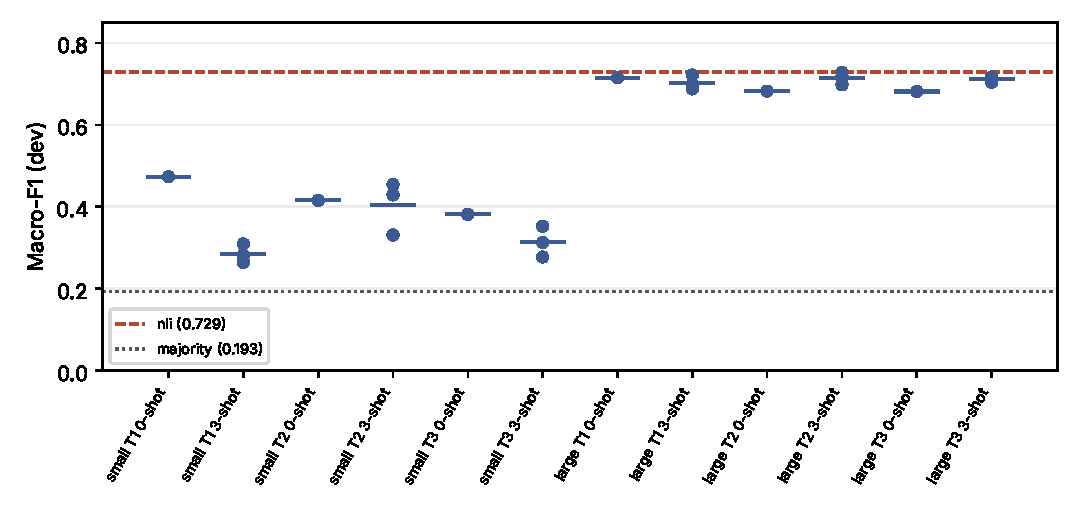
\includegraphics[width=0.8\textwidth]{figures/macro_f1_by_config.pdf}
\caption{Macro-F1 per language-model configuration (dots: individual runs; bar: mean). Dashed line: NLI. Dotted line: majority floor.}\label{fig:f1}
\end{figure*}

\inputifexists{tables/table1_main.tex}{Table 1: main comparison}

\subsection{Handling of NOT ENOUGH INFO}
Table~\ref{tab:nei} shows how often NEI pairs are answered correctly. NLI has NEI recall 0.831 and a confident-wrong rate of 0.169. The 7B model has recall 0.877--0.885 zero-shot (confident-wrong 0.115--0.123); three examples lower recall to 0.710 (T1), 0.774 (T2) and 0.800 (T3) and raise NEI precision from 0.650--0.687 to 0.783--0.827, so the model says NEI less often but is right more often when it does. The 1.5B model rarely abstains correctly: NEI recall is 0.077--0.331 and the confident-wrong rate is at least 0.669; in the T1 and T3 three-shot runs, 302 to 329 of the 340 prediction rows are SUPPORT.

The abstention sentence that distinguishes T3 from T2 did not help. For the 7B model NEI recall changes from 0.877 to 0.885 (zero-shot) and from 0.774 to 0.800 (three-shot), and macro-F1 is unchanged (0.682 vs 0.682 and 0.714 vs 0.712). For the 1.5B model NEI recall falls (0.315$\to$0.231 zero-shot, 0.321$\to$0.097 three-shot) and macro-F1 falls by 0.034 and 0.091. NLI has the lowest ECE (0.145), against 0.220--0.252 for the 7B model and 0.220--0.380 for the 1.5B model; the ECE of the language models rests on first-token label probabilities.
\inputifexists{tables/table2_nei.tex}{Table 2: NEI handling}

\subsection{Numeric claims}
Table~\ref{tab:numeric} compares error rates on numeric and other pairs. The gap (numeric minus other, seed-13 run) ranges from $-0.077$ to $+0.027$, and all 14 intervals, including NLI and the majority floor, contain zero; the intervals are 0.18--0.23 wide. However, the hand check described in Section~III shows that the tag is not valid: of the 11 sampled claims it tagged numeric, only 1 states a quantity, and the other 10 contain digits inside names such as APOE4, p53 or UBC13 (by my reading of the sample). The ``numeric'' group in Table~\ref{tab:numeric} is therefore mostly a group of claims that mention such names, and the table does not show whether numeric claims are easier or harder. The rule also missed a claim about incidence rates. A fair test needs a corrected tag, applied and logged as a post-hoc change, and a larger hand-checked sample.
\inputifexists{tables/table3_numeric.tex}{Table 3: numeric versus other claims}
\figifexists{figures/error_numeric_vs_other.pdf}{Error rate on numeric and other claims, first seed of each configuration.}{fig:numeric}

\subsection{Error analysis}
I read the full abstracts for a random sample of 20 wrong predictions from each of the zero-shot T2 runs (seed 13) of the 7B and the 1.5B model. The counts below describe these samples only, not the full error sets; confusion matrices for whole runs are in \texttt{results/figures}.

\emph{7B model.} In 12 of 20 sampled errors the model answered NEI although the pair has evidence (8 gold CONTRADICT, 4 gold SUPPORT); 7 were direction errors between SUPPORT and CONTRADICT (4 gold CONTRADICT labelled SUPPORT, 3 gold SUPPORT labelled CONTRADICT); 1 NEI pair was labelled SUPPORT. For two claims about the same abstract on macrolides and myocardial infarction (one gold SUPPORT, one gold CONTRADICT), the model answered NEI for both, with NEI probabilities of 0.98 and 0.86.

\emph{1.5B model.} In 12 of 20 sampled errors an NEI pair was labelled SUPPORT, in 1 labelled CONTRADICT; 6 gold-CONTRADICT pairs were labelled SUPPORT and 1 NEI. For two claims about the same abstract, ``cold exposure increases BAT recruitment'' and ``cold exposure reduces BAT recruitment'' (both gold NEI), the model labelled both SUPPORT (probabilities 0.83 and 0.65), so it did not separate opposite claims. Several NEI pairs labelled SUPPORT are statements that sound plausible in general (for example about ivermectin and onchocerciasis, or obesity and quality of life); this fits an account in which the model agrees with plausible claims instead of checking the abstract, but I did not test that account.

\section{Discussion}
\emph{What the data show.} (i) A zero-shot NLI cross-encoder matches the 7B model within the available uncertainty and clearly beats the 1.5B model. (ii) Three examples do not help uniformly: they lowered the 1.5B model's score in all three templates and moved the 7B model from NEI towards CONTRADICT (its CONTRADICT F1 rose from 0.51--0.59 to 0.62--0.64 while NEI recall fell). (iii) The abstention sentence of T3 did not raise NEI recall in either model. (iv) No error-rate gap was detected between rule-tagged numeric pairs and other pairs, but the tag was found invalid (precision 1/11 on 30 hand-checked claims), so nothing can be said about numeric claims.

\emph{Possible explanations (not tested).} The 1.5B model's drift to SUPPORT with examples may be a prior towards agreeing with the claim; because the three examples always appear in the order SUPPORT, CONTRADICT, NEI, an order effect is also possible, and neither was tested. The lack of effect from the abstention sentence may mean that small models do not follow such instructions reliably, or that the label definitions already in T2 carried the information.

\emph{What the data cannot show.} They do not show that NLI is better than the 7B model, whether numeric claims are easier or harder, or anything about retrieval, full texts or other fields, because the correct abstract is always given.

\section{Limitations}
The relevant abstract is given to every method, so the results say nothing about retrieval or about open-domain use. Evidence is limited to abstracts. The study covers one biomedical dataset and cannot support claims about other scientific fields. SciFact is public and may have appeared in the pretraining data of the models, which I cannot check. Only dev labels are available, so dev serves as the final evaluation set; to avoid tuning on it, prompt design used training examples only. The numeric tag is a simple rule that over-tags dataset names with digits, and the numeric subset may be small, which widens the intervals. The NLI-to-NEI mapping is an assumption. NEI pairs here are abstracts that a claim cites but that contain no evidence for it; this construction \cite{kumar2026} may differ from other NEI definitions, and whether such abstracts are easier or harder than random abstracts was not tested. Quantisation of the larger model may change its behaviour, and I did not measure the effect. Results depend on three fixed prompts and three seeds. The seeds select the three-shot examples only, and the same three example sets (one pair per label, always shown in the order SUPPORT, CONTRADICT, NEI) are used for both language models and all templates, so ``seed'' and ``example set'' cannot be separated. Of the nine example abstracts, three also occur in the dev split (one for seed 13, two for seed 42, none for seed 2026), although no example claim does; the seed with no overlap has the lowest three-shot macro-F1 in five of the six model--template combinations, which is consistent with a benefit from overlap but is not evidence of one. Zero-shot settings have a single run. The numeric tag failed its hand check (precision 1/11, recall 1/2 on 30 claims), and 30 claims with only 2 true numeric ones is too few to estimate recall well. The stored ECE is computed from first-token label probabilities and is not comparable across model families without care.

\section{Conclusion}
On 339 SciFact dev pairs with the correct abstract supplied, a zero-shot NLI cross-encoder (macro-F1 0.729) and Qwen2.5-7B-Instruct in 4-bit (0.682--0.715) cannot be told apart at this sample size, Qwen2.5-1.5B-Instruct is much weaker and often collapses to SUPPORT with three examples, and an explicit instruction to answer NEI when unsure did not raise NEI recall. No error-rate gap was detected for rule-tagged numeric claims, but the tag mostly marks digits in names (precision 1/11 on 30 hand-checked claims), so the study cannot say whether numeric claims are harder. What was not measured: retrieval, full-text evidence, other domains, and the effect of quantisation. Useful follow-ups are a corrected numeric tag with a larger hand-checked sample, and more few-shot example sets with the example order varied.

\section*{Use of AI Assistance}
I used Claude (Anthropic) as an assistant for planning the study, drafting code and unit tests, debugging, auditing the saved results by re-scoring them, and drafting the text of this paper. I reviewed and edited the output, ran the experiments myself, and the reported numbers come from the code outputs in the repository. The prompt log and the corrections I made are in \texttt{ai\_assistance\_log.md}.

\bibliographystyle{IEEEtran}
\bibliography{references}

\end{document}